% !TeX program = pdflatex
% !BIB program = bibtex
\documentclass[10pt,conference,letterpaper]{IEEEtran}

\usepackage[T1]{fontenc}
\usepackage[utf8]{inputenc}
\usepackage{amsmath,amssymb}
\usepackage{booktabs}
\usepackage{cite}
\usepackage{graphicx}
\usepackage{siunitx}
\usepackage{tabularx}
\usepackage{tikz}
\usetikzlibrary{arrows.meta,positioning}
\usepackage{xurl}
\usepackage[hidelinks]{hyperref}
\urlstyle{same}
\sisetup{detect-all=true}
\hypersetup{
  pdftitle={Channel Knowledge Maps for FR3 UAV Base Stations: Dataset and ML-Based Modeling},
  pdfauthor={Guillem Moreno Garcia, Sergi Abadal, Evgenii Vinogradov}
}

\title{Channel Knowledge Maps for FR3 UAV Base Stations: Dataset and ML-Based Modeling}

\author{\IEEEauthorblockN{Guillem Moreno Garcia, Sergi Abadal, Evgenii Vinogradov}
\IEEEauthorblockA{Universitat Polit\`ecnica de Catalunya (UPC), Barcelona, Spain\\
guillem.moreno.garcia@estudiantat.upc.edu}}

\begin{document}
\maketitle

\begin{abstract}
This paper introduces a dense FR3 channel knowledge map (CKM) dataset for
unmanned aerial vehicle base stations. It contains 16180 ray-traced
layout--height combinations from 3236 urban locations in 66 cities at
\SI{7.125}{GHz}. Every $513\times513$ realization stores building geometry,
geometric visibility, attenuation, delay spread, angular spread, and a
variable transmitter height. As a focused first benchmark, we propose an
interpretable height-aware attenuation model. Its line-of-sight branch combines
free-space loss with a coherent image-source two-ray term and compact
height/range calibration. Its non-line-of-sight branch combines a
COST231-shaped basis with local morphology and topology-specific linear
calibration. Under a strict city holdout, the frozen model reaches
\SI{1.9289}{dB} overall root mean square error, with \SI{1.7370}{dB} in LoS and
\SI{3.5363}{dB} in NLoS, on 2590 maps from 14 unseen cities. Its median CPU
time is \SI{0.0602}{s} per map. The result provides a transparent attenuation
baseline and a physical anchor for later distribution-aware refinement of all
three channel quantities.
\end{abstract}

\begin{IEEEkeywords}
channel attenuation, channel knowledge map, delay spread, path loss, radio
map, unmanned aerial vehicle.
\end{IEEEkeywords}

\section{Introduction}
Uncrewed aerial vehicles (UAVs) carrying base stations can support future 6G
networks through mobility and an increased probability of line of sight (LoS).
Their deployment nevertheless requires fast, location-dependent channel
information for placement and resource management. Channel knowledge maps
(CKMs) address this need by indexing channel information by transmitter or
receiver location~\cite{ckmtutorial2024,zengx2021ckm}.

Dense CKMs can be measured or simulated. Measurements are costly to collect at
scale, whereas deterministic ray tracing (RT) provides spatially complete
labels at substantial computational cost. Learned surrogates such as
RadioUNet and PMNet therefore use convolutional encoder--decoders to predict
dense maps from city geometry and transmitter information
\cite{radiounet2020,pmnet2023}. Existing datasets, however, predominantly use
fixed terrestrial transmitters and omit spatially varying building height.
That combination is insufficient for elevated transmitters, whose visibility
and propagation change strongly with altitude. It is especially relevant in
FR3, where the 7--24 GHz range is being studied as a coverage/capacity bridge
for 6G~\cite{Cui2024}.

\begin{table*}[t]
\centering
\caption{Comparison of dense CKM and radio-map datasets.}
\scriptsize
\setlength{\tabcolsep}{4pt}
\begin{tabular}{@{}lcccc@{}}
\toprule
Property & This work & UrbanRadio3D~\cite{radiodiff3d2026} & RadioMapSeer~\cite{dataset2212} & CKMImageNet~\cite{ckmimagenet2025} \\
\midrule
Variable elevated Tx height & yes & no & no & no \\
Layout groups or maps & 3236 groups & 701 & 701 & 40000 \\
Raster size(s) & $513^2$ & $256^2$ & $256^2$ & $32^2$--$128^2$ \\
Horizontal resolution & 1 m & 1 m & 1 m & 2 m \\
Channel quantities & Att. (PL), LoS, DS, AS & PL, DoA, ToA & PL & Gain, AoA/AoD, delay \\
Building-height raster included & yes & yes & no & no \\
Per-sample topology labels & 3 and 6 classes & no & no & no \\
\bottomrule
\end{tabular}
\label{tab:datasets}
\vspace{-8pt}
\end{table*}

Table~\ref{tab:datasets} compares released learning inputs rather than the
provenance of the source geometry. Here, 3236 location groups paired with five
transmitter heights produce 16180 realizations. ``Building-height raster''
means that every building pixel retains a height, rather than only a binary
footprint; it does not imply that every height was surveyed directly. We
combine global products providing both footprint and height
\cite{Che2024globfp,Zhu2025atlas}, avoiding the sparse height tags in
OpenStreetMap~\cite{Bernard2022}.

RadioUNet introduced image-to-image dense radio-map regression with a U-Net-like
architecture that encodes building geometry and transmitter location
\cite{radiounet2020}. PMNet subsequently increased convolutional capacity for
the same broad task~\cite{pmnet2023}, while more recent work uses
generative models to represent fine spatial detail and uncertainty
\cite{radiodiff3d2026}. These models are appropriate when propagation effects
cannot be summarized by a low-dimensional base, but their reported errors and
costs depend strongly on raster support, transmitter protocol, target scaling,
and split construction. A number copied across those contracts is therefore
context, not a controlled ranking.

The GLOBECOM 2025 sample reviewed for this paper confirms the breadth of the
current design space: two-stage diffusion~\cite{tsrdiff2025}, a heterogeneous
multitask Gaussian process~\cite{rohmtgp2025}, a large masked transformer
\cite{genspectralm2025}, a variational U-Net~\cite{radiovae2025}, self-supervised
encoder--decoder pretraining~\cite{sslradio2025}, and a distribution-aware
masked autoencoder~\cite{krmae2025}. Most do not disclose enough dimensions or
sampling details for an exact per-map operation count. We therefore use those
works to establish the architectural trend, and reserve quantitative
complexity comparisons for executable models or a complete published layer
table.

This work occupies a complementary point in that design space. The model is
ML-based because all lookup tables and ridge coefficients are learned from
training cities, but its hypothesis class is deliberately constrained: a
coherent field handles repeatable LoS rings, and linear morphology features
handle NLoS structure. This separation makes the stable component auditable and
cheap, and leaves a physically anchored residual for a later neural refiner.
The dataset is released with the richer channel targets needed to test that
refinement under one common geometry and city holdout.

\begin{figure*}
\centering

\includegraphics[width=\textwidth]{figures/ckm_dataset_real_sample.png}
\caption{One released Barcelona realization (\texttt{sample\_02806}) at
$h_{\mathrm{tx}}=\SI{69.4}{m}$. The left illustration shows an elevated UxNB
above six aligned $513\times513$ rasters. The panels show building height,
building mask, LoS, attenuation, delay spread, and angular spread. Crosses mark
the centered transmitter; gray areas are building pixels excluded from the
metrics. For this sample, the stored three- and six-class labels are
\texttt{dense\_highrise} and \texttt{dense\_block\_midrise}.}
\label{fig:ckm_sample}
\vspace{-6pt}
\end{figure*}

Increasingly expressive neural CKM estimators are valuable when sparse
measurements or unresolved effects must be inferred, but their complexity is
rarely isolated from stable propagation structure. We instead ask how much of
the dense field can be captured by a compact physical/statistical base before
learned residual refinement. The contributions are:
\begin{enumerate}
    \item An FR3 CKM dataset from 3236 locations in 66 cities, with five
    transmitter heights per location and aligned attenuation, LoS, delay
    spread, angular spread, building geometry, and topology labels.
    \item A height-aware attenuation model separating coherent LoS structure
    from topology-calibrated NLoS morphology. Every fitted quantity is frozen
    before evaluation on unseen cities.
\end{enumerate}
The released data contain all three channel quantities; this first benchmark
focuses on attenuation.

\section{CKM: Definition and Dataset Description}
\label{sec:ckm_dataset}

For realization $n$, let $\mathbf E_n\in\mathbb R^{H\times W\times L}$
contain environmental layers, $\mathbf C_n\in\mathbb R^{H\times W\times F}$
contain channel quantities, and $\mathbf m_n\in\mathbb R^K$ contain scalar or
categorical metadata. CKM estimation seeks a mapping
\begin{equation}
\widehat{\mathbf C}_n=\mathbf\Phi_{\boldsymbol\theta}
(\mathbf E_n,\mathbf m_n),
\label{eq:mapping_generic}
\end{equation}
where $\boldsymbol\theta$ denotes the estimator parameters. Here $H=W=513$,
$L=2$, and $F=4$. The environmental tensor contains
\begin{enumerate}
    \item a building-height raster $\mathbf H$ in metres, with zero over
    ground; and
    \item a binary building mask $\mathbf B$.
\end{enumerate}
GlobalBuildingAtlas and 3D-GloBFP supply the source building geometry
\cite{Che2024globfp,Zhu2025atlas}. The channel tensor, generated with MATLAB
RT, stores
\begin{enumerate}
    \item binary geometric visibility $\mathbf V$ (LoS $=1$, NLoS $=0$),
    \item attenuation in dB,
    \item RMS delay spread in ns, and
    \item RMS angular spread in degrees.
\end{enumerate}
Building pixels are excluded from training and evaluation. The metadata contain
the centered transmitter height and stored three- and six-class morphology
labels. The attenuation benchmark later recomputes an ITU-inspired three-class
route from each raster; it does not use city identity or channel targets.

The 3236 locations span 66 cities and five independently sampled transmitter
heights each, yielding $N=16180$ realizations. The observed height range is
approximately \SIrange{12}{478}{m}; the receiver height is fixed at
\SI{1.5}{m}. Table~\ref{tab:rt_params} summarizes the common simulation
contract, and Fig.~\ref{fig:ckm_sample} shows a released realization. The
distributed \nolinkurl{CKM_Dataset_270326_labeled.h5} stores both original
topology partitions and the transmitter-height bin alongside the six rasters.

\begin{table}[t]
\centering
\caption{Dataset simulation parameters.}
\label{tab:rt_params}
\scriptsize
\setlength{\tabcolsep}{4pt}
\begin{tabular}{ll}
\toprule
Parameter & Value \\
\midrule
Carrier frequency & \SI{7.125}{GHz} \\
Antenna model & Isotropic \\
Map and resolution & $513\times513$ at \SI{1}{m} \\
Ground receiver height & \SI{1.5}{m} \\
Observed transmitter height & \SIrange{12}{478}{m} \\
Heights per location & 5 \\
Locations / realizations & 3236 / 16180 \\
\bottomrule
\end{tabular}
\end{table}

\section{Height-Aware CKM Modeling}\label{sec:ckm_model}

Fig.~\ref{fig:CKM_model} summarizes the proposed attenuation-focused mapping.
Only compact lookup tables and linear weights are learned, and all are frozen
before a held-out city is evaluated.
\begin{figure}[t]
\centering
\resizebox{\columnwidth}{!}{%
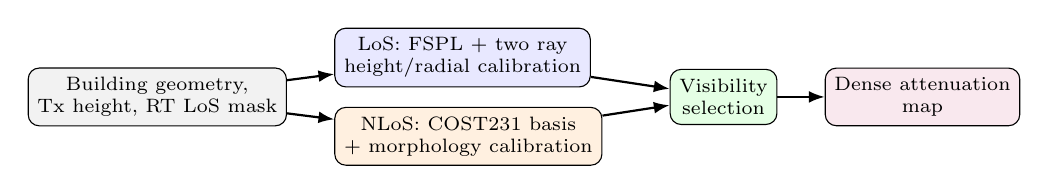
\begin{tikzpicture}[
node distance=5mm and 6mm,
box/.style={draw,rounded corners,align=center,minimum height=7mm,font=\scriptsize},
arr/.style={-{Latex[length=2mm]},thick}]
\node[box,fill=gray!10] (input) {Building geometry,\\Tx height, RT LoS mask};
\node[box,fill=blue!9,right=of input,yshift=5mm] (los) {LoS: FSPL + two ray\\height/radial calibration};
\node[box,fill=orange!12,right=of input,yshift=-5mm] (nlos) {NLoS: COST231 basis\\+ morphology calibration};
\node[box,fill=green!10,right=10mm of los,yshift=-5mm] (switch) {Visibility\\selection};
\node[box,fill=purple!9,right=of switch] (out) {Dense attenuation\\map};
\draw[arr] (input) -- (los);
\draw[arr] (input) -- (nlos);
\draw[arr] (los) -- (switch);
\draw[arr] (nlos) -- (switch);
\draw[arr] (switch) -- (out);
\end{tikzpicture}}
\caption{Separate LoS and NLoS mechanisms are calibrated on training cities.}
\label{fig:CKM_model}
\end{figure}

On valid ground receivers, the stored visibility mask $\mathbf V$ selects
\begin{equation}
\boldsymbol\Lambda=\mathbf V\odot\boldsymbol\Lambda_{\mathrm{LoS}}
 +(1-\mathbf V)\odot\boldsymbol\Lambda_{\mathrm{NLoS}}.
\label{eq:combined}
\end{equation}
The mask is the configured MATLAB ray tracer's own binary visibility output,
not a prediction of the attenuation model. For horizontal distance $d_{2D}$,
the direct and image-source distances are
$d_{3D}=[d_{2D}^2+(h_{\mathrm{tx}}-h_{\mathrm{rx}})^2]^{1/2}$ and
$d_{\mathrm{GR}}=[d_{2D}^2+(h_{\mathrm{tx}}+h_{\mathrm{rx}})^2]^{1/2}$.

\subsection{LoS Branch}
The LoS model retains the phase difference between direct and reflected paths:
\begin{align}
\Lambda_{\mathrm{FSPL}}&=20\log_{10}(4\pi d_{3D}f/c),\label{eq:fspl}\\
C_{\mathrm{2ray}}&=-20\log_{10}\left|1+\rho(h_{\mathrm{tx}})
\frac{d_{3D}}{d_{\mathrm{GR}}}
e^{-j[k(d_{\mathrm{GR}}-d_{3D})+\phi(h_{\mathrm{tx}})]}\right|,\label{eq:tworay}\\
\Lambda_{\mathrm{LoS}}&=\Lambda_{\mathrm{FSPL}}+C_{\mathrm{2ray}}
+\beta(h_{\mathrm{tx}})+r(d_{2D},h_{\mathrm{tx}}).\label{eq:pl_los}
\end{align}
Here $k=2\pi f/c$; $\rho$ and $\phi$ are effective calibration terms rather
than material Fresnel parameters. In each \SI{5}{m} training-height bin, a
small grid search tests $\rho\in\{0,0.05,\ldots,1.5\}$ and 48 phases in
$[-\pi,\pi)$. For each pair, the closed-form mean residual gives $\beta$; the
pair minimizing LoS RMSE is retained. A smoothed radial table $r$ then stores
the remaining mean residual by distance. Neighboring height entries are
linearly interpolated at inference. This captures the repeatable interference
rings without memorizing two-dimensional building texture~\cite{rappaport}.

\subsection{NLoS Branch}
For NLoS receivers, a COST231/Hata-derived urban expression is used only as an
inspectable basis function because its source domain does not cover the
present frequency or heights~\cite{cost231}. With
$d_{\mathrm{km}}=\max(d_{2D}/\SI{1000}{m},0.001)$,
$f_{\mathrm{MHz}}=7125$, and $h_{\mathrm{rx}}=\SI{1.5}{m}$,
\begin{align}
\widetilde\Lambda_C={}&46.3+33.9\log_{10}f_{\mathrm{MHz}}
-13.82\log_{10}h_{\mathrm{tx}}-a(h_{\mathrm{rx}})\nonumber\\
&+(44.9-6.55\log_{10}h_{\mathrm{tx}})\log_{10}d_{\mathrm{km}}+3,\label{eq:cost}\\
a(h_{\mathrm{rx}})={}&(1.1\log_{10}f_{\mathrm{MHz}}-0.7)h_{\mathrm{rx}}\nonumber\\
&-(1.56\log_{10}f_{\mathrm{MHz}}-0.8).
\end{align}
The regression feature is $\Lambda_C=\operatorname{clip}
(\widetilde\Lambda_C,0,185)$.

Let $\mathbf G=1-\mathbf B$ mark ground and
$\mathbf N=(1-\mathbf V)\odot\mathbf G$ mark NLoS ground. For a
reflect-padded $k\times k$ box mean $\mathcal A_k$, $k\in\{15,41\}$, define
\begin{equation}
\begin{gathered}
\ell_d=\ln(1+d_{2D}/\SI{1}{m}),\qquad
\delta_k=\mathcal A_k[\mathbf B],\\
h_k=\mathcal A_k[\mathbf H\odot\mathbf B]/\SI{90}{m},\qquad
n_k=\mathcal A_k[\mathbf N],\\
\theta_n=\operatorname{clip}(\theta/90,0,1),\\
\sigma_{\mathrm{sh}}=2.3197[\max(90-\theta,0)]^{0.2361},
\end{gathered}
\label{eq:features}
\end{equation}
where $\theta$ is the elevation angle in degrees and
$\sigma_{\mathrm{sh}}$ is a deterministic angular feature, not a random
shadowing realization. The implemented vector is
\begin{equation}
\begin{aligned}
\mathbf x=[&\Lambda_C,\ell_d,\delta_{15},\delta_{41},h_{15},h_{41},
\delta_{41}\ell_d,n_{15},n_{41},\\
&n_{41}\ell_d,\sigma_{\mathrm{sh}},\theta_n,n_{41}\theta_n,1]^\top .
\end{aligned}
\label{eq:nlos-vector}
\end{equation}

Routing is computed from each height raster. With building set $\mathcal B$,
$N_b$ four-connected footprints of area $A$ in \si{km^2}, and one maximum
height $H_j$ per footprint, we estimate
\begin{equation}
\hat\alpha=\frac{|\mathcal B|}{513^2},\quad
\hat\beta=\frac{N_b}{A},\quad
\hat\gamma=\sqrt{\frac{1}{2N_b}\sum_{j=1}^{N_b}H_j^2}.
\label{eq:itu-routing}
\end{equation}
The minimum equal-weight log-ratio distance to the ITU-inspired
$(\alpha,\beta,\gamma)$ prototypes suburban $(0.1,750,8)$, urban
$(0.3,500,15)$, dense urban $(0.5,300,20)$, and urban high-rise
$(0.5,300,50)$ assigns the route, with high-rise merged into dense urban
\cite{iturp1410,saboor2024geometry}. The transmitter height regimes are low
for $h_{\mathrm{tx}}\le\SI{60}{m}$, middle for
$\SI{60}{m}<h_{\mathrm{tx}}\le\SI{100}{m}$, and high for
$h_{\mathrm{tx}}>\SI{100}{m}$. This gives nine topology/height regimes without
a city-name lookup.

For each training map, at most 1024 NLoS pixels are selected deterministically.
Non-intercept features are standardized within regime $q$ and fitted by
\begin{equation}
\hat{\mathbf w}_q=\arg\min_{\mathbf w}\sum_{i\in q}
(\mathbf z_i^\top\mathbf w-y_i)^2+10^{-2}\|\mathbf w_{\neg b}\|_2^2.
\label{eq:nlos-ridge}
\end{equation}
The deployed NLoS estimate is
\begin{equation}
\Lambda_{\mathrm{NLoS}}=\operatorname{clip}
(\mathbf x^\top\hat{\mathbf w}_q,20,185).
\label{eq:nlos-output}
\end{equation}
The intercept is unpenalized. In the second expression, the coefficients have
been transformed back to raw feature space.

\section{Results}\label{sec:results}

\subsection{Protocol}
The city holdout contains 10840 maps from 37 training cities, 2750 from 15
validation cities, and 2590 from 14 final-test cities. Calibration uses
training cities only; validation is reserved for development and ablation.
Buildings are excluded before receiver statistics or metrics are computed.
The test set contains 545568250 ground locations, of which 28.199\% are NLoS
according to the RT visibility mask. The metric further removes 122481131
ground locations without a target in the stored $[20,185]$ dB support. Among
the remaining 423087119 receivers, 7.413\% are NLoS. Although the
pixel-weighted score is therefore LoS dominated, 424 test maps contain more
than 25\% valid NLoS receivers.

For valid mask $m_i(p)$, estimate $\hat y_i(p)$, and target $y_i(p)$, the
headline error is
\begin{equation}
\mathrm{RMSE}=\sqrt{\frac{\sum_i\sum_p m_i(p)
[\hat y_i(p)-y_i(p)]^2}{\sum_i\sum_p m_i(p)}}.
\label{eq:rmse}
\end{equation}
Uncertainty uses 20000 percentile-bootstrap draws over held-out cities, not
pixels, thereby preserving within-city spatial dependence.

\begin{figure}[t]
\centering

\includegraphics[width=\columnwidth]{figures/nlos_heldout_example.png}
\caption{Held-out Vancouver \texttt{sample\_15262}
($h_{\mathrm{tx}}=\SI{50.30}{m}$; urban, low-height regime). Columns compare
the CKM dataset target with the model output; rows show all valid receivers,
LOS, and NLOS. Gray marks buildings in the first row and receivers outside the displayed
visibility subset below; building pixels never enter the metrics. The map has
119180 LOS and 25607 NLOS receivers. Full, LOS, and NLOS RMSE are 2.18, 2.10,
and \SI{2.52}{dB}, respectively.}
\label{fig:nlos-example}
\end{figure}

\subsection{Ablation and Accuracy}
Validation ablation confirms that the coherent reflected field is essential:
adding it to FSPL with height bias reduces LoS RMSE from 3.7900 to
\SI{1.7412}{dB}, while the radial table changes it only to
\SI{1.7388}{dB}. In NLoS, training-only global calibration reduces the raw
COST231-basis RMSE from 25.4045 to \SI{3.2179}{dB}; observable topology/height
routing reaches \SI{3.1983}{dB}. Thus, calibration explains the main NLoS
reduction, while routing provides a smaller refinement.

\begin{table}[t]
\centering
\caption{Frozen test metrics; intervals resample 14 cities.}
\label{tab:main-results}
\scriptsize
\setlength{\tabcolsep}{4pt}
\begin{tabular}{lcc}
\toprule
Metric & Estimate & 95\% interval \\
\midrule
Overall RMSE [dB] & 1.9289 & [1.7985, 2.0960] \\
Overall MAE [dB] & 1.2170 & [1.1371, 1.3177] \\
LoS RMSE [dB] & 1.7370 & [1.6603, 1.8225] \\
NLoS RMSE [dB] & 3.5363 & [3.2335, 3.8482] \\
Macro-city RMSE [dB] & 1.9831 & [1.8495, 2.1297] \\
\bottomrule
\end{tabular}
\end{table}

On final test, the complete model reaches \SI{1.9289}{dB} overall RMSE and
\SI{1.2170}{dB} MAE; LoS and NLoS RMSE are 1.7370 and \SI{3.5363}{dB}.
A 20000-draw city bootstrap gives a 95\% overall-RMSE interval of
\SIrange{1.7985}{2.0960}{dB}. Per-city RMSE ranges from \SI{1.6149}{dB} in
Halifax to \SI{2.5851}{dB} in Osaka, with an unweighted mean of
\SI{1.9831}{dB}.

To separate model compactness from routing, Table~\ref{tab:routing-ablation}
recalibrates every retained feature set on training cities before frozen test
evaluation. Relative to the global 14-feature fit, topology-only routing
retains 64\% of the complete routing gain, whereas height-only routing retains
31\%; these shares are not additive because the complete model includes their
interaction. Thus, topology is the stronger routing partition on final test.
The eight-feature model
$[\Lambda_C,\ell_d,\delta_{41},h_{41},n_{41},\sigma_{\mathrm{sh}},
\theta_n,1]$ retains over 90\% of the complete model's reduction from a
single global NLoS constant. A topology-specific constant is already a useful
\SI{4.5391}{dB} NLoS baseline, but it is essentially tied with the global
constant; topology helps primarily through its fitted slopes rather than its
intercept alone.

\begin{table}[t]
\centering
\caption{Frozen test NLoS ablation; every row is recalibrated.}
\label{tab:routing-ablation}
\scriptsize
\setlength{\tabcolsep}{3.2pt}
\begin{tabular}{lccr}
\toprule
Variant & Routing & Terms & RMSE [dB] \\
\midrule
Complete & topology $\times$ height & 14 & 3.5363 \\
Topology only & topology & 14 & 3.5437 \\
Height only & height & 14 & 3.5504 \\
Global fit & none & 14 & 3.5568 \\
41-pixel compact & topology $\times$ height & 8 & 3.5642 \\
Without 15-pixel scale & topology $\times$ height & 11 & 3.5443 \\
Without 41-pixel scale & topology $\times$ height & 8 & 3.6352 \\
Without local morphology & topology $\times$ height & 5 & 3.6907 \\
Topology constant & topology & 1 & 4.5391 \\
Global constant & none & 1 & 4.5403 \\
\bottomrule
\end{tabular}
\end{table}

The scale removals provide a second compactness check. Removing the 15-pixel
summaries changes little, whereas removing the 41-pixel summaries causes the
largest single-scale degradation. Eliminating all local morphology degrades
further. Regional context is therefore useful even though the strong regime
and geometry baseline makes its incremental effect look modest.

Table~\ref{tab:breakdown} uses the same low, middle, and high thresholds as the
fitted model. Error decreases with height, particularly in NLoS. The topology
rows also show materially different propagation regimes: dense urban NLoS is
hardest, while suburban maps are most accurate. The fitted coefficient vectors
change substantially across topologies, so one global set of slopes would mix
distinct relationships; individual coefficients are correlated and are not
interpreted as causal importance scores.

\begin{table}[!t]
\centering
\caption{Pixel-weighted test RMSE [dB] by fitted regime.}
\label{tab:breakdown}
\scriptsize
\setlength{\tabcolsep}{3.5pt}
\begin{tabular}{lrrrr}
\toprule
Regime & Maps & Overall & LoS & NLoS \\
\midrule
Low height & 899 & 2.1437 & 1.7923 & 3.7526 \\
Middle height & 773 & 1.9682 & 1.7747 & 3.5080 \\
High height & 918 & 1.7117 & 1.6697 & 2.7620 \\
\midrule
Suburban & 1455 & 1.6977 & 1.6048 & 3.1632 \\
Urban & 940 & 2.2963 & 1.9967 & 3.6466 \\
Dense urban & 195 & 2.5716 & 2.1126 & 4.1319 \\
\midrule
All & 2590 & 1.9289 & 1.7370 & 3.5363 \\
\bottomrule
\end{tabular}
\end{table}

\begin{table}[t]
\centering
\caption{Selected raw-space NLoS coefficients, middle height.}
\label{tab:nlos-coefficients}
\scriptsize
\setlength{\tabcolsep}{3.1pt}
\begin{tabular}{lrrr}
\toprule
Feature & Suburban & Urban & Dense urban \\
\midrule
$\Lambda_C$ & 0.1458 & 0.1736 & 0.1617 \\
$\ell_d$ & 4.5443 & 2.6421 & 0.3887 \\
$\delta_{41}$ & -29.8064 & -33.8643 & -33.5577 \\
$n_{41}$ & 19.6343 & 3.9023 & -13.4237 \\
$\sigma_{\mathrm{sh}}$ & -10.9186 & -10.6507 & -10.4005 \\
$\theta_n$ & -20.0207 & -20.4908 & -29.2653 \\
Bias & 136.6540 & 141.6217 & 155.0450 \\
\bottomrule
\end{tabular}
\end{table}

Table~\ref{tab:nlos-coefficients} makes the topology dependence explicit.
For example, the regional blocked-ground coefficient is positive in suburban
and urban maps but negative in dense urban maps. Such sign changes arise from
jointly fitted, correlated regressors; they need not mean that one physical
effect reverses in isolation. They do show that the fitted relationship, not
only its intercept, differs by morphology.

\begin{table}[t]
\centering
\caption{Reported RMSE [dB]. Only the first two rows share a test contract.}
\label{tab:accuracy-context}
\scriptsize
\setlength{\tabcolsep}{1.5pt}
\begin{tabular}{@{}>{\raggedright\arraybackslash}p{1.55cm}>{\raggedright\arraybackslash}p{1.95cm}rrr@{}}
\toprule
Method & Evaluation contract & All & LoS & NLoS \\
\midrule
Proposed & CKM city holdout & 1.9289 & 1.7370 & 3.5363 \\
GMM U-Net & Same split and masks & 4.3606 & 4.4323 & 3.3381 \\
RadioUNet \cite{radiounet2020} & RadioMapSeer DPM & 1.60 & -- & -- \\
RadioVAE$_C$ \cite{radiovae2025} & RadioMapSeer DPM & 1.42 & -- & -- \\
TSRDiff \cite{tsrdiff2025} & BRAT-Lab, 10\% samples & 3.62 & -- & -- \\
RO-HMTGP \cite{rohmtgp2025} & Measured RSRP & 4.19--6.00 & -- & -- \\
\bottomrule
\end{tabular}
\vspace{-4pt}
\end{table}

The GMM U-Net is a controlled neural alternative: a height-conditioned mixture
head and U-Net decoder, separated into six topology classes and LoS/NLoS
experts, are evaluated on the same 2590 maps and receiver masks. It is the best
purely neural approach found in an internal exploration of over 50 model
configurations. Its lower NLoS error shows where distribution-aware learning
can help, while the substantially lower LoS and overall errors of the proposed
model show the value of resolving the stable coherent component explicitly.
This neural result is included as a preview, not as the final hybrid: a
following paper will train neural models to refine the calibrated priors for
attenuation, delay spread, and angular spread.

The remaining rows are published context, not a controlled ranking. RadioUNet
reports 0.020 gray-level RMSE, or \SI{1.60}{dB} under its 80-dB scaling;
RadioVAE$_C$ reports 0.0177, or \SI{1.42}{dB}, without input measurements
\cite{radiounet2020,radiovae2025}. Both use $256^2$ fixed-height terrestrial
RadioMapSeer data. TSRDiff uses sparse target measurements, and RO-HMTGP
predicts measured RSRP across six cells rather than dense simulated
attenuation. Their reported
RMSE values therefore indicate scale under different tasks, not superiority
over the present $513^2$ variable-height city holdout.

\subsection{Computational Comparison}
Table~\ref{tab:compute} uses the same AMD Ryzen 5 5600X, six CPU threads, batch
one, and GPU-disabled execution for the proposed model and neural baselines.
The neural timings use official implementations, 10 warmups, and 50 forward
passes; input and file I/O are excluded.

\begin{table}[!t]
\centering
\caption{Computational context; reported CPU rows use the same CPU.}
\label{tab:compute}
\scriptsize
\setlength{\tabcolsep}{2.2pt}
\begin{tabular}{@{}lcrrr@{}}
\toprule
Method & Grid & State & Reported MAC & CPU [s] \\
\midrule
Proposed & $513^2$ & 66.8k+126 & 0.170M$^\ast$ & 0.0602 \\
RadioUNet~\cite{radiounet2020} & $256^2$ & 13.27M & 12.73G & 0.1339 \\
PMNet~\cite{pmnet2023} & $256^2$ & 33.34M & 52.71G & 0.4042 \\
SSL-Radio~\cite{sslradio2025} & $256^2$ & 15.4--20.4M & 16.9--21.9G$^\dagger$ & -- \\
MATLAB RT & $513^2$ & -- & -- & 102.289 \\
\bottomrule
\end{tabular}
\end{table}
The asterisk counts the final 14-term NLoS dot product averaged over valid
test NLoS pixels; feature construction and lookup operations are additional.
The dagger is reconstructed from SSL-Radio's layer table under two plausible
skip-concatenation interpretations, rather than measured from released code.
The proposed timing includes feature construction and LoS evaluation. MATLAB
R2024b takes a median \SI{102.289}{s} over five Barcelona layouts with one
reflection and no diffraction on the same CPU. RT also produces visibility
and all three channel quantities, so the raw $\sim1700\times$ difference is
not a like-for-like speedup. It nevertheless demonstrates a significant
computational gap for the attenuation prior.

\subsection{Scope and Limitations}
The reported accuracy is conditional on the supplied RT visibility mask. For
fixed city geometry, transmitter position and height, receiver grid, and RT
settings, that mask is deterministic and can be stored once; a repeated
five-condition audit found all 742392 receiver visibility values identical.
This is not a claim that an independently reconstructed mask is interchangeable
with the stored one. The fitted tables also inherit the simulator, isotropic
antenna, fixed carrier, flat terrain, and building products used to create the
data. COST231 supplies only a calibrated basis outside its original domain,
and the model does not identify the particular reflected or diffracted NLoS
path. These constraints are why the result is presented as a transparent
dataset baseline and refinement anchor, not as a universal propagation law.

\section{Conclusions}\label{sec:conclusions}
We introduced a dense FR3 UAV CKM dataset containing attenuation, delay
spread, angular spread, visibility, building geometry, transmitter height, and
topology labels for 16180 realizations from 66 cities. The accompanying
attenuation benchmark separates coherent LoS structure from calibrated NLoS
morphology and freezes every fitted quantity before unseen-city evaluation.
It reaches \SI{1.9289}{dB} overall RMSE while remaining compact, auditable, and
fast on a CPU. The results further show that topology is the principal NLoS
calibration partition, with transmitter height refining that partition and
the regional morphology scale carrying most of the useful local context.

The model is intended as a physical/statistical base rather than a rejection
of deep learning. The controlled GMM U-Net result identifies NLoS as the
promising refinement target, but also shows the cost of asking a network to
relearn the coherent LoS field. A future journal paper will instead train
distribution-aware networks to refine analogous calibrated priors for
attenuation, delay spread, and angular spread. Its multi-output runtime will
not be directly comparable to this attenuation-only benchmark, but the present
computational gap shows that the prior-first strategy is significant and worth
preserving.

\bibliographystyle{IEEEtran}
\bibliography{references}

\end{document}
